\documentclass[12pt,fleqn]{article}\usepackage{../../common}
\begin{document}
Hamiltonian dinamik - 1

Legendre transformasyonu

E�er size tek bir de�i�kene ba�l� bir fonksiyon verirsem, bu fonksiyona
bakman�n iki yolu var. Biri her $x$ degeri icin onun eslendigi bir $f(x)$
degeri oldugu. Boylece fonksiyonu tanimlamis oluyorum. 

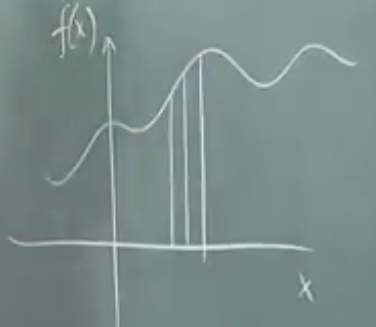
\includegraphics[width=15em]{phy_hamiltonian_1_01.png}

Bir di�eri her noktay� ayn� fonksiyonun {\em e�imine} e�lemek. Tabii bunu
yap�nca �zg�n bir e�leme elde etmi� olmam, $f(x)+4$ ve $f(x)+10$ ayn�
$f'(x)$ e�imine sahip ama bir ba�lang�� referans noktas� da tan�mlarsam,
ana fonksiyonu yakalam�� olurum. Mesela $f(0)$'i tan�mlarsam bu referans
i�ini g�r�r. 

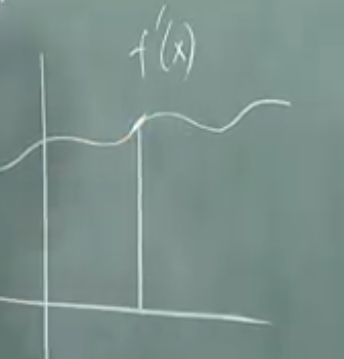
\includegraphics[width=15em]{phy_hamiltonian_1_02.png}

Legendre transformasyonunun arkas�ndaki fikir budur. �stteki �rnek tek
de�i�ken i�in bu durumda ortaya pek fayda g�remiyoruz ama �ok de�i�kenli
ortamda teknik �ok faydal�.



















\end{document}
